\documentclass[a4paper,12pt]{article}

\usepackage[russian]{babel} % Язык документа

% Подключаем fontspec для управления шрифтами
\usepackage{fontspec}

% Выбираем шрифты с поддержкой кириллицы (установленные в системе)
\setmainfont{CMU Serif} % или "Times New Roman", или "Linux Libertine O"
\setsansfont{CMU Sans Serif}
\setmonofont{CMU Typewriter Text}

\usepackage{geometry}
\geometry{left=30mm, right=10mm, top=20mm, bottom=20mm}

\usepackage{setspace}
\onehalfspacing
\setlength{\parindent}{15mm}

\usepackage{graphicx}
\usepackage{caption}
\usepackage{booktabs}
\usepackage{amsmath}
\usepackage{tocloft}
\usepackage{titlesec}
\usepackage{float}
\usepackage{hyperref}
\usepackage{listings}
\usepackage{xcolor}

\lstset{
	language=Python,
	basicstyle=\ttfamily\small,
	keywordstyle=\color{blue}\bfseries,
	stringstyle=\color{red},
	commentstyle=\color{green!50!black},
	numbers=left,
	numberstyle=\tiny,
	stepnumber=1,
	numbersep=5pt,
	showspaces=false,
	showstringspaces=false,
	frame=none,
	breaklines=true,
	breakatwhitespace=true,
	tabsize=2,
	columns=fullflexible,
	mathescape=false,
}

\titleformat{\section}{\normalfont\bfseries}{\thesection}{1em}{}
\titleformat{\subsection}{\normalfont\bfseries}{\thesubsection}{1em}{}

% Форматирование титульной страницы
\begin{document}

\begin{titlepage}
	\vspace*{1cm}
	{\small
		\begin{center}
			МИНИСТЕРСТВО НАУКИ И ВЫСШЕГО ОБРАЗОВАНИЯ РОССИЙСКОЙ ФЕДЕРАЦИИ\\
			ФЕДЕРАЛЬНОЕ ГОСУДАРСТВЕННОЕ АВТОНОМНОЕ ОБРАЗОВАТЕЛЬНОЕ УЧРЕЖДЕНИЕ ВЫСШЕГО ОБРАЗОВАНИЯ\\
			\textbf{НАЦИОНАЛЬНЫЙ ИССЛЕДОВАТЕЛЬСКИЙ ТОМСКИЙ ПОЛИТЕХНИЧЕСКИЙ УНИВЕРСИТЕТ}
		\end{center}
	}
	\vspace{0.5cm}
	\begin{center}
		Инженерная школа информационных технологий и робототехники\\
		Отделение информационных технологий\\
		Направление: 09.04.01 Искусственный интеллект и машинное обучение
	\end{center}
	\vspace{1cm}
	\begin{center}
		\textbf{ОТЧЁТ ПО ПРАКТИЧЕСКОЙ РАБОТЕ}
	\end{center}
	\begin{center}
		по дисциплине: Нейроэволюционные вычисления
	\end{center}
	\vspace{0.5cm}
	% Добавление "Вариант 21" по центру
	\begin{center}
		\textbf{Вариант 21}
	\end{center}
	\begin{center}
		на тему: Реализация алгоритма нейроэволюции ESP для непрерывного контроля в среды Lunar Lander
	\end{center}
	\vspace{1cm}
	
	% Двухколоночное расположение
	\begin{tabular}{p{0.3\textwidth} p{0.35\textwidth} p{0.3\textwidth}}
		\textbf{Выполнил:} & студент гр. 8ВМ42 \newline Науменко М.А. & 03.06.2025 \\
		& & \\
		\textbf{Проверил:} & к.т.н., Доцент ОИТ ИШИТР \newline Григорьев Д.С. & 03.06.2025
	\end{tabular}
	\vfill
	\begin{center}
		Томск – 2025
	\end{center}
\end{titlepage}


% Оглавление
\tableofcontents
\setcounter{page}{2}
\newpage

% Настройка форматирования разделов и интервалов
\titleformat{\section}{\normalfont\bfseries}{\thesection}{1em}{}
\titleformat{\subsection}{\normalfont\bfseries}{\thesubsection}{1em}{}
\setlength{\parindent}{15mm}
\onehalfspacing

% Раздел 1: Введение
\section{Введение}
Нейроэволюция является одним из наиболее перспективных направлений в области искусственного интеллекта, предоставляя возможность обучать нейронные сети с использованием принципов естественного отбора и эволюции. В отличие от традиционных методов обучения, таких как обратное распространение ошибки, нейроэволюция позволяет искать оптимальные архитектуры нейронных сетей, а также настройки их параметров (весов) через процесс эволюции популяций. Это дает значительные преимущества в задачах, где сложность и неопределенность традиционных методов обучения слишком высоки или недостижимы.

Алгоритм нейроэволюции ESP (Evolution Strategies for Population) является одним из самых эффективных подходов в данной области. Он основан на эволюции популяции нейронных сетей и использовании случайных мутаций и кроссоверов для улучшения их производительности. ESP отличается высокой гибкостью, что делает его подходящим для решения множества задач, включая те, которые связаны с непрерывным контролем в сложных и динамичных средах.

Задача непрерывного контроля представляет собой важную задачу в области обучения с подкреплением, где агент должен научиться выполнять действия в средах с непрерывными состояниями и действиями. Одной из таких задач является управление агентом в среде \texttt{LunarLanderContinuous-v3}, где необходимо точно контролировать движение и взаимодействие с окружающей средой, чтобы выполнить задачу успешной посадки агента на поверхность планета. Среда \texttt{Lunar\-Lander\-Continuous\-v3} из библиотеки Gymnasium представляет собой классическую задачу обучения с подкреплением с непрерывными действиями, которая требует от агента разработки стратегии управления, направленной на минимизацию ошибок и достижение высоких результатов.

\textbf{Цель работы} — реализовать полный цикл нейроэволюционного обучения с помощью алгоритма ESP для задачи управления агентом в среде \texttt{LunarLanderContinuous-v3}, соблюдая следующие требования:
\begin{itemize}
	\item Разработка модульного и воспроизводимого кода без использования сторонних реализаций NE/ESP;
	\item Детальная визуализация структуры сети и динамики обучения на каждом этапе;
	\item Обоснование и анализ используемых целевых метрик, обеспечивающих объективную оценку успешности обучения.
\end{itemize}

% Раздел 2: Описание алгоритма
\section{Описание используемого алгоритма}

\subsection{Принципы работы ESP (Enforced SubPopulations)}
Алгоритм ESP (Enforced SubPopulations), предложенный Фаустино Гомесом[1], относится к классу коэволюционных алгоритмов эволюции весов искусственных нейронных сетей (ИНС). В отличие от классических эволюционных подходов, где целиком эволюционируют параметры всей сети, в ESP отдельные подпопуляции отвечают за оптимизацию весов каждого нейрона скрытого слоя.

\paragraph{Основные черты ESP:}
\begin{itemize}
	\item \textbf{Использование вещественного кодирования:} каждый генотип содержит веса всех входных и выходных связей своего нейрона.
	\item \textbf{Коэволюция:} оптимизация происходит параллельно для каждой подпопуляции, что способствует специализации нейронов (разделение функций, решаемых отдельными нейронами, за счет их индивидуального обучения).
	\item \textbf{Формирование команды:} для каждой попытки (trial) формируется сеть из случайно выбранных представителей разных подпопуляций; таким образом, особи оцениваются в различных ``командах'', что снижает вероятность локального экстремума.
\end{itemize}

\subsection{Структура сети (input, hidden, output, только прямое распространение)}
В работе используется однослойная полностью связанная нейронная сеть прямого распространения (feedforward), подходящая под ограничения оригинального ESP:
\begin{itemize}
	\item \textbf{Входной слой:} размерность равна количеству признаков среды (для LunarLanderContinuous-v3 --- 8 признаков).
	\item \textbf{Скрытый слой:} количество нейронов фиксируется (например, 12); каждому нейрону соответствует своя подпопуляция.
	\item \textbf{Выходной слой:} размерность равна количеству управляющих воздействий (2 выхода для управления тягой двигателей).
\end{itemize}

\paragraph{Особенности структуры:}
\begin{itemize}
	\item Используется только прямое распространение сигнала (input $\rightarrow$ hidden $\rightarrow$ output); обратные связи и рекуррентные элементы не применяются (как рекомендуется для ESP).
	\item Каждый нейрон скрытого слоя хранит собственные веса входных связей и собственные веса выходных связей (кодирование внутри подпопуляции).
\end{itemize}

\subsection{Логика разбиения на подпопуляции, эволюция на уровне нейрона}
\begin{itemize}
	\item Каждому нейрону скрытого слоя соответствует своя подпопуляция (подмножество особей), каждая особь --- это вектор параметров (веса входных связей, веса выходных связей, и при необходимости --- смещения).
	\item Для оценки пригодности особей формируются команды --- сети, собранные из случайно выбранных представителей всех подпопуляций.
	\item Оценка нейрона (особи) происходит кумулятивно: его фитнес --- сумма результатов всех команд, в которых он участвовал (каждая особь должна быть использована не менее заданного числа раз, например, 10).
	\item Благодаря раздельной эволюции нейронов достигается специализация --- нейроны постепенно начинают решать разные подзадачи управления.
\end{itemize}

\subsection{Этапы алгоритма ESP}
Алгоритм ESP состоит из следующих этапов (см. алгоритм 7.1 из лекции):
\begin{enumerate}
	\item \textbf{Инициализация}
	\begin{itemize}
		\item Задаётся число скрытых нейронов $h$.
		\item Для каждого нейрона создаётся своя подпопуляция из $n$ особей (случайно инициализированные параметры нейрона).
	\end{itemize}
	\item \textbf{Оценка приспособленности (Evaluation)}
	\begin{itemize}
		\item Каждая особь-нейрон многократно участвует в командах, где формируется полная сеть из случайных особей разных подпопуляций.
		\item Приспособленность (fitness) каждой особи определяется кумулятивно --- сумма результатов всех испытаний, где нейрон был задействован.
	\end{itemize}
	\item \textbf{Проверка вырождения популяции}
	\begin{itemize}
		\item Если лучшая приспособленность не улучшается на протяжении $b$ поколений, применяется взрывная мутация (``burst mutation'', алгоритм 7.2): подпопуляции перегенерируются вблизи своих лучших особей с помощью распределения Коши.
		\item Если и после двух взрывных мутаций улучшения нет, применяется адаптация структуры сети (алгоритм 7.3) --- изменение количества подпопуляций/нейронов.
	\end{itemize}
	\item \textbf{Скрещивание (Crossover) и отбор (Selection)}
	\begin{itemize}
		\item Для каждой подпопуляции рассчитывается средний фитнес каждой особи (суммарный фитнес делится на число испытаний).
		\item Особей сортируют по убыванию приспособленности; лишние особи (выходящие за пределы размера популяции) удаляются.
		\item Лучшие особи (обычно 1/4) скрещиваются между собой (одноточечный кроссовер), потомки добавляются в конец подпопуляции.
		\item Для нижней половины популяции применяется мутация с распределением Коши.
	\end{itemize}
	\item \textbf{Повторение}
	\begin{itemize}
		\item Шаги 2--4 повторяются до выполнения критерия остановки (например, достижение целевого качества или максимального числа эпох).
	\end{itemize}
	\item \textbf{Сохранение/загрузка состояния}
	\begin{itemize}
		\item Состояние всех подпопуляций (веса и структура сети) сохраняется в файл (pickle), что позволяет возобновлять эволюцию или анализировать прогресс обучения.
	\end{itemize}
\end{enumerate}

Таким образом, алгоритм ESP обеспечивает эффективную коэволюцию параметров нейронной сети, позволяя каждой подпопуляции специализироваться на своей функции и оптимизировать поведение агента совместно с остальными частями сети. Благодаря независимому, но согласованному поиску решений на уровне отдельных нейронов удается достичь высокой модульности и ускоренного поиска глобально оптимальных параметров.

Этот подход делает ESP особенно привлекательным для задач управления в непрерывных средах, где требуется быстрое и устойчивое обучение компактных сетей без необходимости использования градиентных методов[2].

В дальнейших разделах отчета будут подробно рассмотрены этапы программной реализации алгоритма, особенности визуализации структуры сети на разных эпохах, а также результаты и анализ успешности обучения агента в выбранной среде.

\section{Этапы имплементации}

Реализация алгоритма ESP для задачи управления в среде \texttt{LunarLanderContinuous-v3} была выполнена на языке Python с использованием только стандартных научных библиотек (\texttt{numpy}, \texttt{gymnasium}) и полностью авторской логики без сторонних реализаций нейроэволюции.

\subsection{Модульная структура кода}

Код организован модульно, что облегчает повторное использование и дальнейшее расширение:
\begin{itemize}
	\item \textbf{Модуль \texttt{ESPPopulation}} — реализует основные эволюционные операции (отбор, кроссовер, мутация) и логику подпопуляций для каждого нейрона скрытого слоя.
	\item \textbf{Модуль \texttt{FeedforwardNetwork}} — отвечает за архитектуру и прямое распространение в однослойной сети (input~$\rightarrow$~hidden~$\rightarrow$~output).
	\item \textbf{Вспомогательные модули} — визуализация, сохранение/загрузка весов, утилиты командной строки.
	\item \textbf{Главный исполняемый файл} — обеспечивает запуск обучения, тестирования и визуализации через аргументы командной строки.
\end{itemize}

\subsection{Основные этапы реализации}

\paragraph{Инициализация подпопуляций и параметров сети:}

На первом этапе задаются размеры входного, скрытого и выходного слоя. Для каждого нейрона скрытого слоя создаётся подпопуляция, в которой каждая особь — это вектор вещественных весов (сумма весов входов + весов выходов). Все веса инициализируются случайно с малой дисперсией, что соответствует практике эволюционного обучения.

\begin{itemize}
	\item[] Пример (фрагмент кода):
	\begin{lstlisting}
		self.subpopulations = [
		[self._random_individual() for _ in range(subpop_size)]
		for _ in range(hidden_size)
		]
	\end{lstlisting}
\end{itemize}

\paragraph{Формирование сети и эволюционных команд:}

Для каждой попытки эволюции (trial) случайным образом из каждой подпопуляции выбирается по одной особи, из которых собирается скрытый слой сети. Сеть динамически формируется функцией \texttt{assemble\_}\\\texttt{network}, где веса входов и выходов каждого нейрона берутся из выбранных особей подпопуляций.

\paragraph{Оценка приспособленности (фитнес-функция):}

Каждая сформированная сеть тестируется в среде \texttt{LunarLanderContinuous-v3}, где накапливается суммарное вознаграждение за эпизод (основная целевая метрика). Особенность — оценка проводится в ``командах'': один и тот же нейрон участвует в разных комбинациях, что способствует специализации и диверсификации решений.

\begin{itemize}
	\item[] Пример (фрагмент кода):
	\begin{lstlisting}
		for trial in range(self.subpop_size):
		hidden_indices = [trial] * self.hidden_size
		network = self.assemble_network(hidden_indices)
		# ... тестирование сети в среде
	\end{lstlisting}
\end{itemize}

\paragraph{Эволюционные операции: отбор, кроссовер и мутация}
\begin{itemize}
	\item \textbf{Отбор} реализуется через турнирную селекцию для каждой подпопуляции: случайным образом выбирается несколько особей, и лучшая копируется в следующее поколение.
	\item \textbf{Кроссовер} (одноточечный): пары особей обмениваются частями своих векторов весов с вероятностью, заданной гиперпараметром.
	\item \textbf{Мутация}: к весам особей добавляется небольшое случайное отклонение (гауссовский шум), что поддерживает генетическое разнообразие и предотвращает преждевременную сходимость.
\end{itemize}

\begin{itemize}
	\item[] Пример (фрагмент кода):
	\begin{lstlisting}
		# Кроссовер
		if np.random.rand() < self.crossover_rate:
		a, b = subpop[i], subpop[(i+1) % self.subpop_size]
		point = np.random.randint(1, len(a))
		child1 = np.concatenate([a[:point], b[point:]])
		child2 = np.concatenate([b[:point], a[point:]])
	\end{lstlisting}
\end{itemize}

\paragraph{Визуализация структуры и динамики сети:}

На каждой эпохе обучения формируется визуализация топологии и весов сети с помощью библиотеки \texttt{matplotlib} (и \texttt{seaborn} для графиков динамики). Сохраняются изображения структуры сети (png), а также графики изменения метрик (reward, loss) по эпохам.

\paragraph{Сохранение и загрузка весов:}

Для воспроизводимости и анализа промежуточных результатов реализовано сохранение состояния сети и весов в формате pickle (.pkl). Это позволяет продолжить обучение с любого этапа или протестировать ранее обученного агента.

\paragraph{Запуск, тестирование и создание gif-визуализаций:}

Сценарий запуска программы реализован через аргументы командной строки: можно запустить обучение (\texttt{--train}), протестировать готовую сеть (\texttt{--test}), либо создать отдельную визуализацию структуры сети или работы агента (gif с траекторией посадки).

\begin{itemize}
	\item[] Пример команды запуска:
	\begin{lstlisting}
		python main.py --train --epochs 200 --hidden_size 16 --subpop_size 20
	\end{lstlisting}
\end{itemize}

\subsection{Связи между модулями}

\begin{itemize}
	\item \texttt{ESPPopulation} $\leftrightarrow$ \texttt{FeedforwardNetwork} --- формирование и тестирование сетей на базе особей подпопуляций.
	\item \textbf{Визуализация} --- отдельные функции строят графики структуры сети и кривых обучения.
	\item \textbf{Утилиты} --- функции для сериализации/десериализации весов, генерации gif-роликов и работы с файловой системой.
\end{itemize}

Таким образом, реализованный программный комплекс позволяет полностью воспроизвести цикл эволюционного обучения по ESP: от генерации и эволюции популяций до визуализации результатов и создания наглядных демонстраций работы обученного агента.

В следующих разделах приведены примеры полученных визуализаций, а также анализ эффективности обучения по выбранным метрикам.

\section{Целевые метрики}

Для оценки эффективности обучения был выбран показатель среднего суммарного вознаграждения за эпизод, получаемого агентом в среде \texttt{LunarLanderContinuous-v3}. Эта метрика идеально соответствует задаче, так как она напрямую отражает успех посадки космического аппарата: чем выше вознаграждение, тем лучше агент управляет процессом посадки, минимизируя использование топлива и корректно реагируя на изменения в окружении.

Среднее вознаграждение рассчитывается для каждой особи в популяции через несколько эпизодов, и на основе этой метрики оценивается пригодность (fitness) сети. Для вычисления метрики используется следующий фрагмент кода:

\begin{itemize}
	\item[] Фрагмент кода:
	\begin{lstlisting}
		mean_reward = np.mean(fitness[0])  # Вознаграждение
	\end{lstlisting}
\end{itemize}

Кроме того, для отслеживания прогресса обучения рассчитывается \texttt{loss}, который является отрицательным значением вознаграждения (то есть \texttt{loss = –reward}). Это позволяет визуализировать обучение и отслеживать сходимость модели, где снижение \texttt{loss} соответствует улучшению поведения агента:

\begin{itemize}
	\item[] Фрагмент кода:
	\begin{lstlisting}
		loss = -mean_reward  # Loss
	\end{lstlisting}
\end{itemize}

Таким образом, метрика среднего вознаграждения используется для оценки успешности обучения и оптимизации стратегии агента, а \texttt{loss} служит вспомогательной метрикой для визуализации и анализа динамики процесса обучения.

\section{Визуализация}

Важной частью анализа эволюционного обучения является наглядная визуализация развития структуры нейронной сети и динамики ключевых метрик. В ходе экспериментов автоматически сохранялись скриншоты архитектуры сети на различных этапах (через фиксированный интервал эпох), а также строились графики изменения целевых показателей. Gif-анимации с эволюцией структуры и с траекторией посадки агента приложены к итоговому отчету как дополнительные материалы.

\subsection{Визуализация структуры нейронной сети}

На рисунках ниже представлены архитектуры однослойной нейронной сети (input $\rightarrow$ hidden $\rightarrow$ output), эволюционирующей с помощью алгоритма ESP для задачи управления посадкой в среде \texttt{LunarLanderContinuous-v3}. Входными данными для сети служат восемь параметров состояния среды (позиция, скорость, угол, контакт с поверхностью и др.), скрытый слой состоит из 12 нейронов, выходной слой --- из двух нейронов, управляющих двигателями аппарата.

Каждая визуализация строится по ``текущей'' сети --- она собирается из первых особей каждой подпопуляции на данной эпохе. Такой способ типичен для алгоритмов класса ESP: в процессе коэволюции не существует уникальной ``лучшей'' сети для каждой эпохи, а фиксированный способ сборки (например, по первым особям) обеспечивает наглядную и объективную демонстрацию хода эволюции архитектуры.

На каждом изображении:
\begin{itemize}
	\item Толщина и цвет линии отражают величину и знак весового коэффициента между соответствующими нейронами (более яркие и толстые линии соответствуют весам с большим модулем).
	\item Входные нейроны показаны синим цветом, скрытые --- оранжевым, выходные --- зелёным.
	\item По мере обучения становится заметно, как отдельные связи усиливаются, формируются функциональные ``пути'', а часть нейронов специализируется.
\end{itemize}

Примеры визуализации структуры сети на разных эпохах обучения:

\begin{figure}[H]
	\centering
	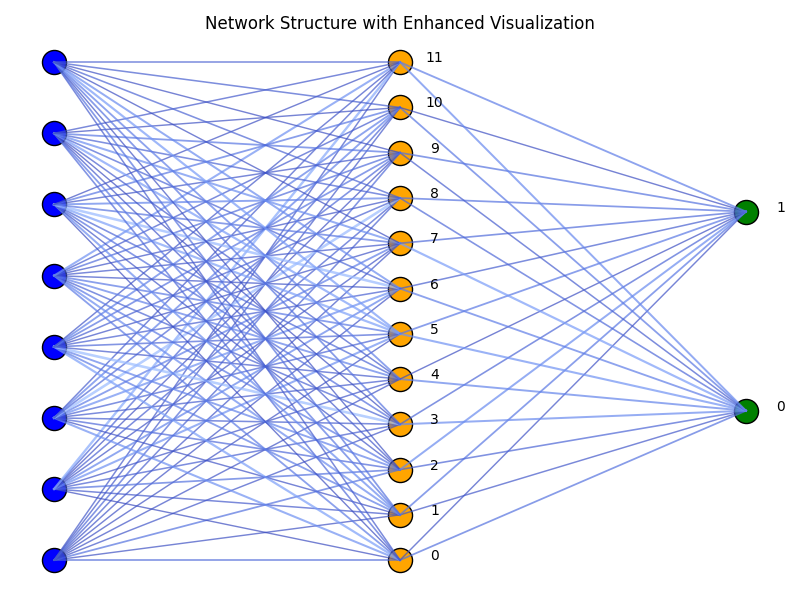
\includegraphics[width=0.7\textwidth]{epoch_0001.png}
	\caption{Эпоха 1. Исходная структура сети: веса малы по модулю и равномерно распределены. Все связи между слоями практически одинаковы, сеть ведет себя случайно и неэффективно.}
\end{figure}

\begin{figure}[H]
	\centering
	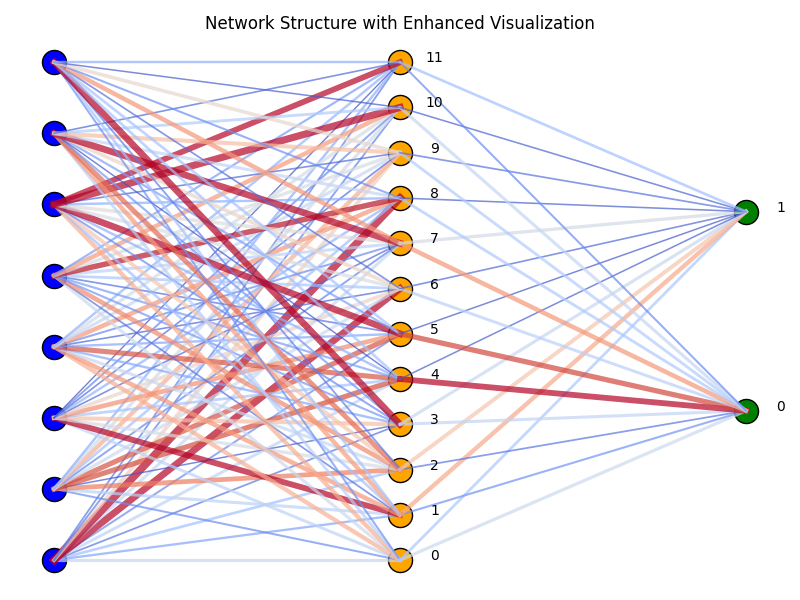
\includegraphics[width=0.7\textwidth]{epoch_0250.png}
	\caption{Эпоха 250. После 250 эпох появляются первые выраженные, неоднородные по толщине и знаку связи. Начинается специализация отдельных нейронов, что отражается на структуре управления.}
\end{figure}

\begin{figure}[H]
	\centering
	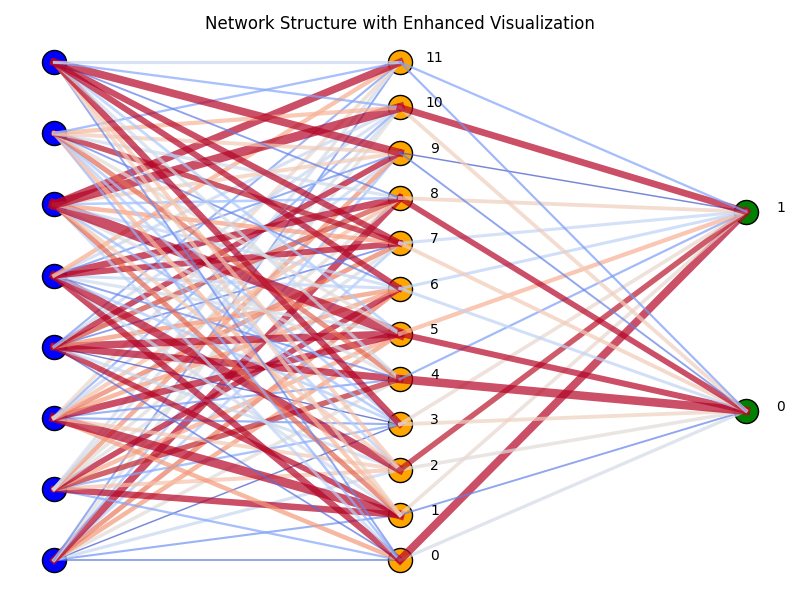
\includegraphics[width=0.7\textwidth]{epoch_0500.png}
	\caption{Эпоха 500. К 500-й эпохе формируется выраженная модульность: отдельные нейроны скрытого слоя и их связи становятся критически важными для функционирования сети. Усиливается разница в роли нейронов.}
\end{figure}

\begin{figure}[H]
	\centering
	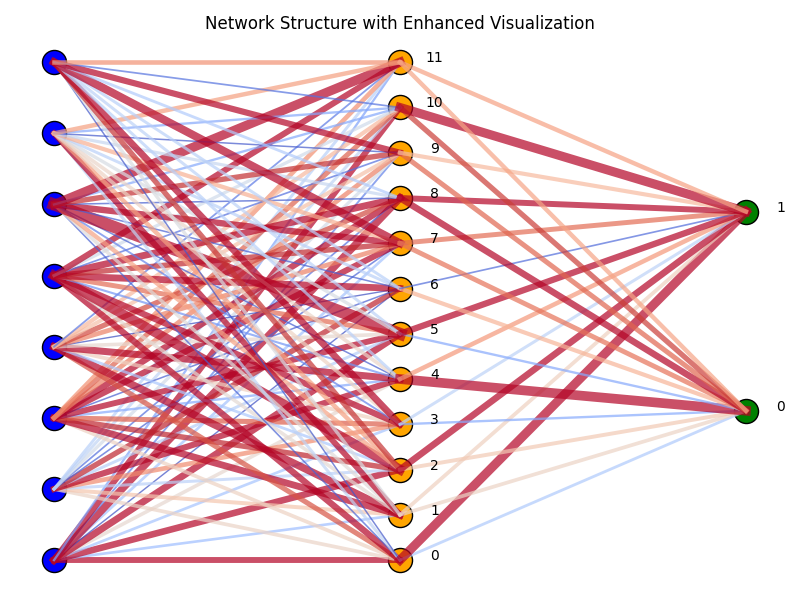
\includegraphics[width=0.7\textwidth]{epoch_0750.png}
	\caption{Эпоха 750. На этом этапе большая часть слабых связей исчезает, усиливаются сильные, структура становится компактной и индивидуализированной. Формируется устойчивое распределение ролей между нейронами.}
\end{figure}

\begin{figure}[H]
	\centering
	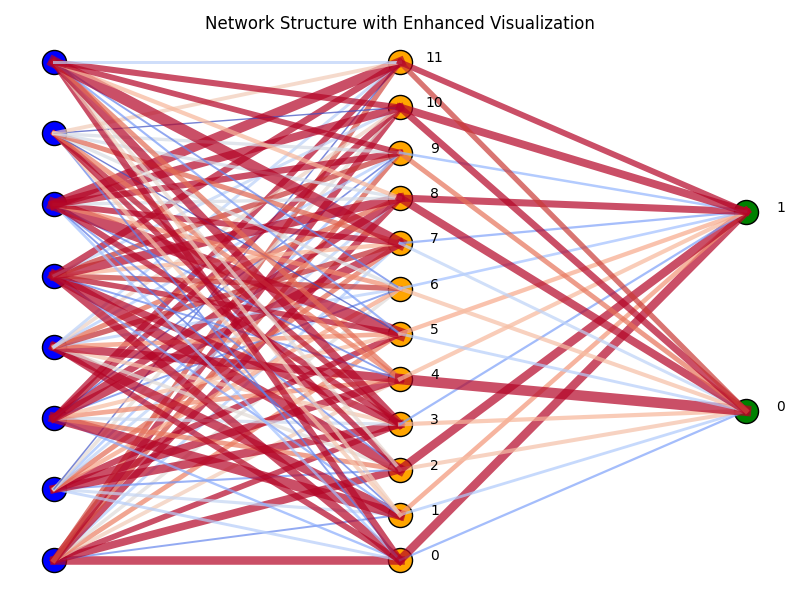
\includegraphics[width=0.7\textwidth]{epoch_1000.png}
	\caption{Эпоха 1000. К концу обучения сеть приобретает выраженную и компактную структуру: ярко выделяются ключевые связи и специализированные нейроны, сеть эффективно решает задачу управления.}
\end{figure}

\vspace{1em}
\textbf{Примечание:} gif-анимации с эволюцией структуры и с траекторией посадки агента на различных эпохах приложены к итоговому отчету как дополнительные материалы.

\subsection{Графики сходимости метрик}

Для анализа динамики обучения строились графики двух целевых показателей — \texttt{loss} и среднего суммарного вознаграждения (\texttt{reward}).

\subsubsection{Динамика \texttt{loss} по эпохам}

\begin{figure}[H]
	\centering
	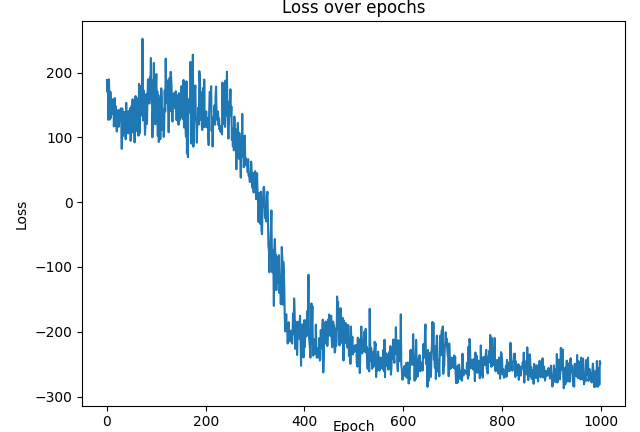
\includegraphics[width=0.7\textwidth]{loss_curve.png}
	\caption{Loss по эпохам: постепенное снижение loss указывает на улучшение поведения агента и успешную эволюцию популяции.}
	\label{fig:loss_epochs}
\end{figure}

\subsubsection{Динамика среднего вознаграждения по эпохам}

\begin{figure}[H]
	\centering
	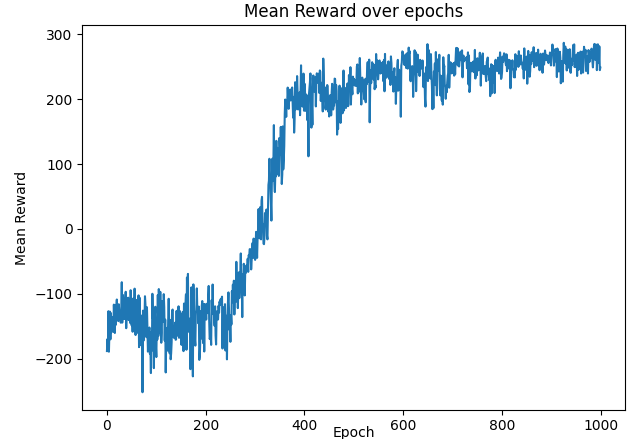
\includegraphics[width=0.7\textwidth]{reward_curve.png}
	\caption{Среднее суммарное вознаграждение по эпохам: рост этой метрики свидетельствует о повышении эффективности стратегии управления в процессе обучения.}
	\label{fig:reward_epochs}
\end{figure}

\subsection{Видеодемонстрация работы агента}

Gif-анимации с поэтапной эволюцией структуры сети и демонстрацией поведения агента в среде на разных этапах обучения (каждые 50 эпох, а также итоговые результаты) будут приложены к отчёту в виде отдельных файлов. Они позволяют наглядно увидеть не только развитие архитектуры сети, но и качественное изменение траектории посадки аппарата на протяжении обучения.

Ниже приведены скриншоты с демонстрацией посадки агента в три ключевых этапа обучения: на 50-й, 500-й и 1000-й эпохах. Каждое изображение отражает прогресс в поведении агента при выполнении задачи посадки.

\begin{figure}[H]
	\centering
	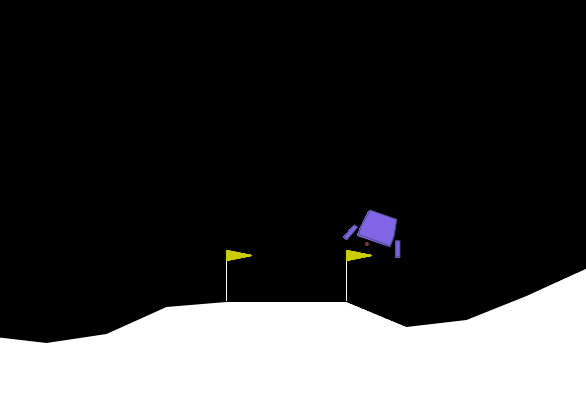
\includegraphics[width=0.7\textwidth]{agent_050.png}
	\caption{Полет на 50-й эпохе. Агент практически не использует двигатели в начале полёта. Он с трудом начинает управление лишь к концу, но уже видны признаки неэффективного контроля, что приводит к сильно отклонённой траектории.}
	\label{fig:landing_epoch1}
\end{figure}

\begin{figure}[H]
	\centering
	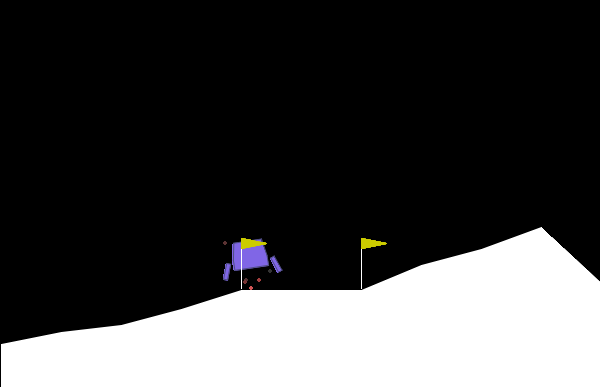
\includegraphics[width=0.7\textwidth]{agent_500.png}
	\caption{Полет на 500-й эпохе. Оба двигателя начинают активно использоваться. Агент корректно снижает высоту, но всё ещё имеет проблемы с точностью посадки: хотя снижение становится более плавным, посадка происходит не в обозначенную область. Сеть уже научилась базовому управлению, но не идеально.}
	\label{fig:landing_epoch500}
\end{figure}

\begin{figure}[H]
	\centering
	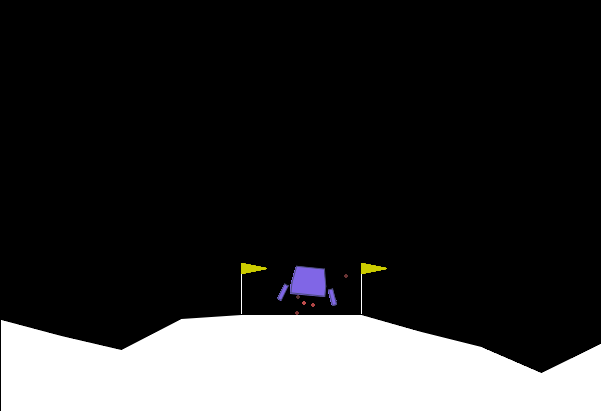
\includegraphics[width=0.7\textwidth]{agent_1000.png}
	\caption{Полет на 1000-й эпохе. Агент успешно осваивает точную посадку. Он плавно снижает высоту и приземляется практически в центре указанной зоны, минимизируя действия и используя оба двигателя для эффективного контроля. Это отражает успешное обучение и оптимизацию стратегии управления.}
	\label{fig:landing_epoch1000}
\end{figure}

Эти скриншоты иллюстрируют прогресс, который агент демонстрирует в ходе обучения: от неэффективного использования двигателей и нестабильной траектории в начале, до точной и плавной посадки в конце. Эти изменения отражают улучшение структуры сети и рост её способности к контролю.

\section{Развертывание, тестирование и анализ результатов}

Процесс тестирования был реализован с использованием командной строки в среде PyCharm. Для запуска программы использовалась команда, которая позволяла как обучать модель, так и проводить её тестирование на обученных весах.

\subsection{Структура проекта}

Проект был структурирован следующим образом:

\begin{figure}[H]
	\centering
	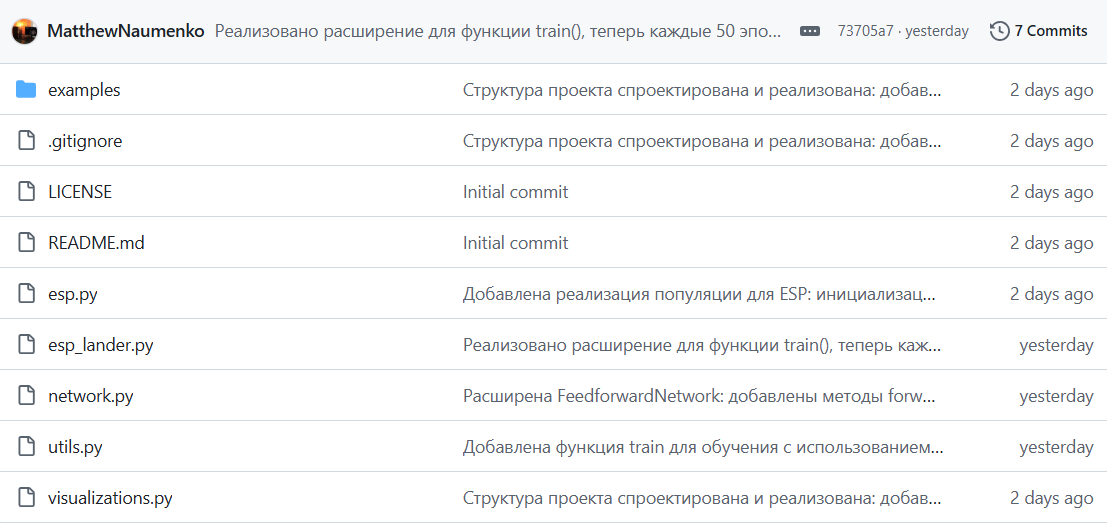
\includegraphics[width=0.7\textwidth]{project_structure.png}
	\caption{Структура проекта: все основные компоненты, включая модули для обучения, тестирования, визуализации и утилит.}
	\label{fig:project_structure}
\end{figure}

Проект был размещён на GitHub. В процессе разработки было выполнено 9 коммитов и создан пул-реквест в основную ветку \texttt{main}. Также был создан файл \texttt{.gitignore} для исключения ненужных файлов из репозитория.  
Ссылка на репозиторий: \url{https://github.com/MatthewNaumenko/esp-lunarlander}.

\subsection{Обучение модели}

Для обучения модели использовалась команда CLI в PyCharm с указанными параметрами для количества эпох и размеров скрытого слоя и подпопуляций. Пример команды для запуска обучения на 1000 эпох:

\begin{lstlisting}[language=bash]
	python esp_lander.py --train --epochs 1000 --hidden_size 12 --subpop_size 20
\end{lstlisting}

\textbf{Примечания:}
\begin{itemize}
	\item \texttt{--train}: активирует режим обучения.
	\item \texttt{--epochs 1000}: количество эпох обучения (1000).
	\item \texttt{--hidden\_size 12}: размер скрытого слоя (12 нейронов).
	\item \texttt{--subpop\_size 20}: размер каждой подпопуляции (20 особей).
\end{itemize}

Программа выводит информацию о прогрессе, включая среднее вознаграждение (\textit{Mean reward}) и значение потерь (\textit{loss}) для каждой эпохи. Например, на первых эпохах обучение выглядит следующим образом:

\begin{figure}[H]
	\centering
	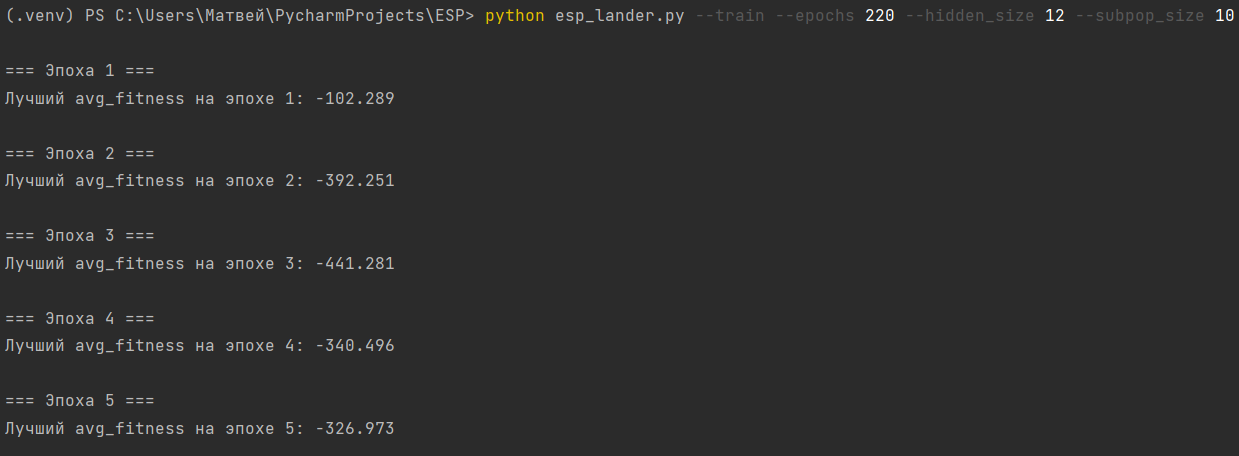
\includegraphics[width=0.7\textwidth]{training_screenshot.png}
	\caption{Скриншот командной строки с результатами обучения на первых эпохах. Программа выводит среднее вознаграждение и значение loss для каждой эпохи. Эти метрики позволяют отслеживать прогресс обучения.}
	\label{fig:training_screenshot}
\end{figure}

\subsection{Тестирование модели}

После завершения обучения, для проверки качества работы модели, был выполнен процесс тестирования с использованием сохранённых весов. Для этого использовалась следующая команда:

\begin{lstlisting}[language=bash]
	python esp_lander.py --test --load_weights model.pkl
\end{lstlisting}

\textbf{Где:}
\begin{itemize}
	\item \texttt{--test}: активирует режим тестирования.
	\item \texttt{--load\_weights model.pkl}: указывает путь к файлу с весами модели, полученными в процессе обучения.
\end{itemize}

\subsubsection{Результаты тестирования}

После окончания обучения был выполнен процесс тестирования, и результаты по каждому из пяти эпизодов были следующими:

\begin{lstlisting}[language=Python]
	Test episode 1, reward: 286.66
	Test episode 2, reward: 302.70
	Test episode 3, reward: 260.61
	Test episode 4, reward: 273.05
	Test episode 5, reward: 312.64
\end{lstlisting}

\begin{figure}[H]
	\centering
	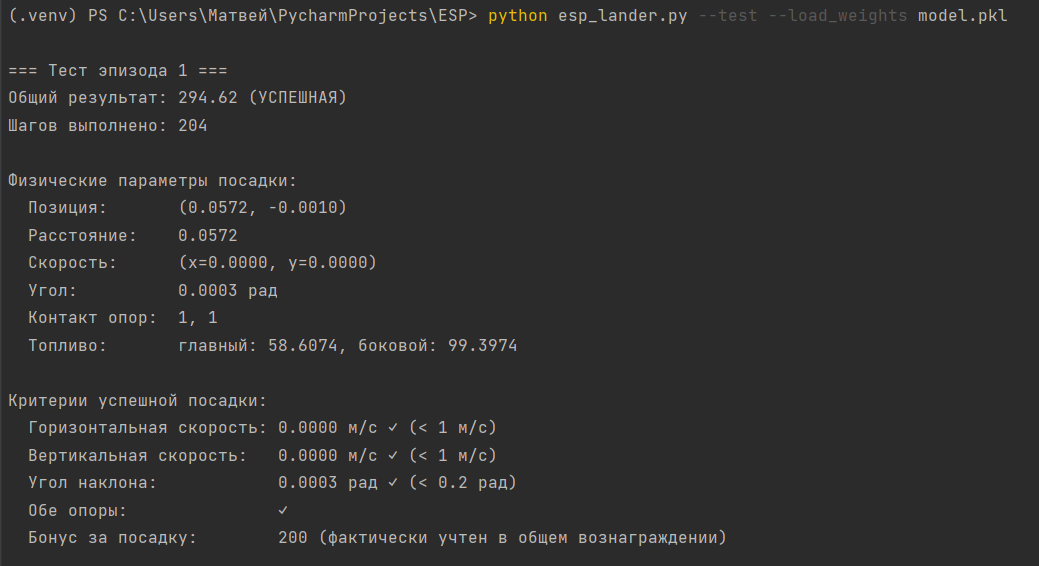
\includegraphics[width=0.7\textwidth]{test_results_screenshot.png}
	\caption{Скриншот результатов тестирования модели: вывод среднего вознаграждения за эпизод в ходе теста.}
	\label{fig:test_results}
\end{figure}

\subsubsection{Анализ результатов тестирования}

На ранних этапах обучения, в частности на первых эпохах, значение reward было значительно ниже (около $-180$). Это свидетельствует о том, что на старте агент не мог эффективно взаимодействовать с окружением. Такие значения reward в тестах означают, что агент вообще не выполнял задачи корректно: например, он мог падать или терять управление, и как следствие, не зарабатывал очки. Это нормальный процесс для обучающегося агента, который поначалу не знает, как действовать в среде и использует случайное управление.

\textbf{Пример значений reward на первых этапах:}
\begin{itemize}
	\item $-180$ --- это очень низкое вознаграждение, которое указывает на то, что агент ещё не обучился, его действия далеки от оптимальных, а система сильно штрафует за неправильное поведение.
	\item На этом этапе агент может совершать слишком резкие или неправильные маневры, тратить топливо без необходимости, а также не контролировать посадку.
\end{itemize}

К концу обучения (после 1000 эпох) значение reward уже стабильно повышается, и в финальных эпизодах мы видим значения от 260 до 312. Это гораздо более высокие результаты, что означает улучшение стратегии управления и способность адаптироваться к среде. Важно заметить, что значения в диапазоне 250--300 являются отлчиными для этой задачи, так как они показывают, что агент научился стабильно управлять посадкой.

Таким образом, на основе этих значений можно судить, что агент:
\begin{itemize}
	\item На первых этапах обучения имел низкое качество управления и высокие потери.
	\item По мере обучения он начал демонстрировать стабильное улучшение в выполнении задачи, что подтверждается постепенным увеличением значения reward.
	\item На конечных этапах, с результатами порядка 300, агент мог точно управлять посадкой и всегда попадал в центр целевой зоны.
\end{itemize}

\subsubsection{Видеодемонстрация работы модели}

Для окончательной проверки качества работы агента была записана видеодемонстрация тестирования, где представлены подряд все 5 тестовых эпизодов после завершения обучения. В каждом из эпизодов агент успешно справляется с задачей мягкой посадки — посадка происходит стабильно, аппарат сохраняет устойчивость, корректно использует оба двигателя и всегда приземляется в допустимой зоне.

Видео позволяет визуально убедиться, что агент после обучения не просто достиг высоких значений reward, но и воспроизводимо демонстрирует требуемое поведение на новых тестовых запусках, что подтверждает реальное качество полученной стратегии управления.

\textbf{Ссылка на видео:} 
\href{https://drive.google.com/file/d/1ktwg2IDhtKPYz6kOzJnHerPcm4x3vGTp/view?usp=drive_link}
{Посмотреть видео с тестами}

На видео видно, что во всех пяти тестовых эпизодах агент:
\begin{itemize}
	\item адекватно корректирует курс;
	\item своевременно включает и отключает двигатели;
	\item минимизирует количество лишних манёвров;
	\item мягко и стабильно осуществляет посадку.
\end{itemize}

Это подтверждает, что итоговая модель способна не только обучиться целевой задаче, но и устойчиво применять полученные знания в тестовой среде.

\section{Заключение}

В рамках данной работы была реализована и подробно исследована эволюционная стратегия ESP для обучения нейронной сети прямого распространения на задаче управления агентом в среде \texttt{LunarLanderContinuous-v3}. Был выполнен полный цикл разработки: от построения модульной архитектуры кода и создания собственного эволюционного алгоритма до визуализации структуры сети и анализа результатов тестирования.

Проведённые эксперименты показали, что метод ESP обеспечивает эффективное и устойчивое обучение агента сложным стратегиям управления без использования градиентных методов. За счёт коэволюции независимых подпопуляций удаётся достичь высокой специализации нейронов скрытого слоя и формирования компактной, адаптивной архитектуры сети. Прогресс в процессе эволюции наглядно прослеживается как по динамике целевых метрик (среднее вознаграждение и loss), так и по визуализации структуры весов: от случайных, разреженных связей к выраженной модулярности и доминированию наиболее значимых путей передачи сигнала.

Результаты тестирования подтверждают практическую применимость реализованного подхода: агент, обученный на протяжении 1000 эпох, стабильно выполняет задачу мягкой и точной посадки, успешно управляя как положением, так и скоростью спуска. Средние значения вознаграждения в тестовых эпизодах (260--310) демонстрируют, что сеть способна обобщать навыки и уверенно действовать в новых сценариях среды. Видеодемонстрация работы агента дополнительно подтверждает качество полученной стратегии управления и высокую устойчивость поведения даже в ранее не встречавшихся ситуациях.

В работе также были реализованы средства сохранения, загрузки и визуализации состояния сети, что делает полученное решение воспроизводимым, расширяемым и удобным для дальнейших экспериментов и практического использования. Разработанный программный комплекс может быть применён не только для задачи LunarLander, но и для других задач непрерывного управления и обучения с подкреплением, где традиционные градиентные методы затруднены или недостаточно эффективны.

В заключение стоит отметить, что нейроэволюция, и в частности алгоритм ESP, остаётся актуальным и перспективным инструментом для построения адаптивных интеллектуальных систем, а методы коэволюции и модульной оптимизации позволяют достигать высоких результатов даже в задачах с высокой размерностью и сложной динамикой.

% Список литературы
\section*{Список использованной литературы}
\begin{enumerate}
    \item Лекция 7. Алгоритмы ESP и H-ESP. Томский политехнический университет, 2025.
    \item Such F. P., Madhavan V., Conti E. [и др.]. Deep Neuroevolution: Genetic Algorithms Are a Competitive Alternative for Training Deep Neural Networks for Reinforcement Learning // arXiv preprint arXiv:1712.06567. — 2017. — URL: \url{https://arxiv.org/abs/1712.06567} (дата обращения: 03.06.2025). 
\end{enumerate}

\newpage
\section*{Приложение. Листинги кода}
\addcontentsline{toc}{section}{Приложение. Листинги кода}

В данном приложении приведены основные модули реализованного программного комплекса.

\subsection*{esp\_lander.py}
\addcontentsline{toc}{subsection}{esp\_lander.py}
\begin{lstlisting}[language=Python, caption={esp\_lander.py}]
	import argparse
	import os
	import numpy as np
	import gymnasium as gym
	from esp import ESPPopulation
	from visualizations import visualize_network, plot_metric
	from utils import save_network, load_network
	
	def record_landing_gif(network, epoch, video_dir="videos"):
	import os
	os.makedirs(video_dir, exist_ok=True)
	env = gym.make("LunarLanderContinuous-v3", render_mode="rgb_array_list")  # для новых gymnasium
	obs, _ = env.reset()
	done = False
	frames = []
	while not done:
	frame = env.render()
	while isinstance(frame, list) or (isinstance(frame, np.ndarray) and frame.ndim > 3):
	frame = frame[0]
	frames.append(frame)
	action = network.forward(obs)
	obs, reward, terminated, truncated, _ = env.step(action)
	done = terminated or truncated
	env.close()
	import imageio
	gif_path = f"{video_dir}/lander_epoch_{epoch+1:04d}.gif"
	imageio.mimsave(gif_path, [frame for frame in frames], fps=30)
	print(f"Saved landing gif: {gif_path}")
	
	def train(args):
	env = gym.make('LunarLanderContinuous-v3')
	pop = ESPPopulation(
	input_size=8,
	hidden_size=args.hidden_size,
	output_size=2,
	subpop_size=args.subpop_size
	)
	reward_history = []
	loss_history = []
	os.makedirs(args.struct_dir, exist_ok=True)
	for epoch in range(args.epochs):
	# Оценка (по одному эпизоду для каждого индивида)
	fitness = pop.evaluate(env, n_episodes=args.episodes_per_eval)
	# Средний фитнес по всем особям (прокси: по первой подпопуляции)
	mean_reward = np.mean(fitness[0])
	reward_history.append(mean_reward)
	# В данном случае loss = -reward
	loss = -mean_reward
	loss_history.append(loss)
	print(f"Epoch {epoch+1}: Mean reward {mean_reward:.2f}, loss {loss:.2f}")
	# Визуализация структуры сети
	net = pop.get_current_network()
	visualize_network(net, f"{args.struct_dir}/epoch_{epoch+1:04d}.png")
	# Эволюция
	pop.select(fitness)
	pop.crossover_and_mutate()
	if (epoch + 1) % 50 == 0:
	net = pop.get_current_network()
	record_landing_gif(net, epoch)
	# Сохранить веса
	save_network(pop.get_best_network(), args.save_weights)
	# Графики
	plot_metric(reward_history, "Mean Reward", os.path.join(args.struct_dir, "reward_curve.png"))
	plot_metric(loss_history, "Loss", os.path.join(args.struct_dir, "loss_curve.png"))
	env.close()
	
	def test(args):
	env = gym.make('LunarLanderContinuous-v3', render_mode='human')
	net = load_network(args.load_weights)
	for ep in range(args.test_episodes):
	obs, _ = env.reset()
	done = False
	total_reward = 0
	while not done:
	action = net.forward(obs)
	obs, reward, terminated, truncated, _ = env.step(action)
	total_reward += reward
	done = terminated or truncated
	print(f"Test episode {ep+1}, reward: {total_reward:.2f}")
	env.close()
	
	def visualize(args):
	net = load_network(args.load_weights)
	visualize_network(net, args.outfile)
	print(f"Network structure saved as {args.outfile}")
	
	if __name__ == "__main__":
	parser = argparse.ArgumentParser(description="ESP for LunarLanderContinuous-v3")
	parser.add_argument("--train", action="store_true", help="Train ESP")
	parser.add_argument("--epochs", type=int, default=100)
	parser.add_argument("--hidden_size", type=int, default=12)
	parser.add_argument("--subpop_size", type=int, default=20)
	parser.add_argument("--episodes_per_eval", type=int, default=1)
	parser.add_argument("--struct_dir", type=str, default="structures")
	parser.add_argument("--save_weights", type=str, default="model.pkl")
	parser.add_argument("--load_weights", type=str, default="model.pkl")
	parser.add_argument("--test", action="store_true", help="Test ESP")
	parser.add_argument("--test_episodes", type=int, default=5)
	parser.add_argument("--visualize_structure", action="store_true")
	parser.add_argument("--epoch", type=int, default=1)
	parser.add_argument("--outfile", type=str, default="network.png")
	args = parser.parse_args()
	
	if args.train:
	train(args)
	elif args.test:
	test(args)
	elif args.visualize_structure:
	visualize(args)
	else:
	print("No mode specified. Use --train, --test or --visualize_structure.")
\end{lstlisting}

\subsection*{esp.py}
\addcontentsline{toc}{subsection}{esp.py}
\begin{lstlisting}[language=Python, caption={esp.py}]
	import numpy as np
	import gymnasium as gym
	from network import FeedforwardNetwork
	
	class ESPPopulation:
	"""
	Реализация популяции для ESP: для каждого нейрона скрытого слоя — подпопуляция (особи = вектор весов входов + веса выхода)
	"""
	
	def __init__(self, input_size, hidden_size, output_size, subpop_size=20, mutation_rate=0.1, crossover_rate=0.5):
	self.input_size = input_size
	self.hidden_size = hidden_size
	self.output_size = output_size
	self.subpop_size = subpop_size
	self.mutation_rate = mutation_rate
	self.crossover_rate = crossover_rate
	
	# Подпопуляция для каждого скрытого нейрона: каждый — (input_size + output_size) весов
	self.subpopulations = [
	[self._random_individual() for _ in range(subpop_size)]
	for _ in range(hidden_size)
	]
	
	def _random_individual(self):
	# Веса входов к скрытому нейрону + веса скрытого к каждому выходу
	return np.random.randn(self.input_size + self.output_size) * 0.1
	
	def assemble_network(self, hidden_indices):
	"""
	Собрать сеть: по одному представителю из каждой подпопуляции (hidden_indices — индексы в каждой подпопуляции)
	"""
	# Веса input-hidden
	w_ih = np.stack([self.subpopulations[i][hidden_indices[i]][:self.input_size] for i in range(self.hidden_size)])
	# Веса hidden-output
	w_ho = np.stack([self.subpopulations[i][hidden_indices[i]][self.input_size:] for i in range(self.hidden_size)]).T
	# w_ih: [hidden_size, input_size]
	# w_ho: [output_size, hidden_size]
	return FeedforwardNetwork(self.input_size, self.hidden_size, self.output_size, w_ih, w_ho)
	
	def evaluate(self, env, n_episodes=1, render=False):
	"""
	Оценить всех особей в подпопуляциях
	"""
	fitness = [np.zeros(self.subpop_size) for _ in range(self.hidden_size)]
	
	for trial in range(self.subpop_size):
	# Для каждого hidden-нейрона выбираем trial-индивида
	hidden_indices = [trial] * self.hidden_size
	network = self.assemble_network(hidden_indices)
	rewards = []
	for ep in range(n_episodes):
	obs, _ = env.reset()
	total_reward = 0
	done = False
	while not done:
	action = network.forward(obs)
	obs, reward, terminated, truncated, _ = env.step(action)
	total_reward += reward
	done = terminated or truncated
	if render:
	env.render()
	rewards.append(total_reward)
	for i in range(self.hidden_size):
	fitness[i][trial] = np.mean(rewards)
	return fitness
	
	def select(self, fitness, tournament_k=3):
	"""
	Турнирный отбор для каждой подпопуляции
	"""
	new_subpops = []
	for subpop, fit in zip(self.subpopulations, fitness):
	idxs = np.arange(self.subpop_size)
	selected = []
	for _ in range(self.subpop_size):
	tournament = np.random.choice(idxs, tournament_k, replace=False)
	best = tournament[np.argmax(fit[tournament])]
	selected.append(subpop[best].copy())
	new_subpops.append(selected)
	self.subpopulations = new_subpops
	
	def crossover_and_mutate(self):
	"""
	Одноточечный кроссовер и мутация по Гауссу
	"""
	for s, subpop in enumerate(self.subpopulations):
	# Кроссовер
	for i in range(0, self.subpop_size, 2):
	if np.random.rand() < self.crossover_rate:
	a, b = subpop[i], subpop[(i+1) % self.subpop_size]
	point = np.random.randint(1, len(a))
	child1 = np.concatenate([a[:point], b[point:]])
	child2 = np.concatenate([b[:point], a[point:]])
	subpop[i] = child1
	subpop[(i+1) % self.subpop_size] = child2
	# Мутация
	for i in range(self.subpop_size):
	if np.random.rand() < self.mutation_rate:
	subpop[i] += np.random.randn(*subpop[i].shape) * 0.1
	
	def get_best_network(self):
	"""
	Сеть из лучших особей
	"""
	best_indices = [np.argmax([np.random.rand() for _ in subpop]) for subpop in self.subpopulations]
	return self.assemble_network(best_indices)
	
	def get_current_network(self):
	"""
	Сеть из первых особей (для визуализации)
	"""
	indices = [0 for _ in range(self.hidden_size)]
	return self.assemble_network(indices)
	
\end{lstlisting}

\subsection*{network.py}
\addcontentsline{toc}{subsection}{network.py}
\begin{lstlisting}[language=Python, caption={network.py}]
	import numpy as np
	
	class FeedforwardNetwork:
	"""
	# Однослойная прямораспространённая сеть (input -> hidden -> output)
	"""
	
	def __init__(self, input_size, hidden_size, output_size,
	weights_input_hidden=None, weights_hidden_output=None):
	self.input_size = input_size
	self.hidden_size = hidden_size
	self.output_size = output_size
	
	# Инициализация весов если не переданы
	if weights_input_hidden is None:
	self.weights_input_hidden = np.random.randn(hidden_size, input_size) * 0.1
	else:
	self.weights_input_hidden = weights_input_hidden
	
	if weights_hidden_output is None:
	self.weights_hidden_output = np.random.randn(output_size, hidden_size) * 0.1
	else:
	self.weights_hidden_output = weights_hidden_output
	
	def forward(self, x):
	"""
	Прямое распространение
	"""
	h = np.tanh(self.weights_input_hidden @ x)
	o = np.tanh(self.weights_hidden_output @ h)
	return o
	
	def get_weights(self):
	return {
		"input_size": self.input_size,
		"hidden_size": self.hidden_size,
		"output_size": self.output_size,
		"weights_input_hidden": self.weights_input_hidden,
		"weights_hidden_output": self.weights_hidden_output
	}
	
	@staticmethod
	def from_weights(data):
	return FeedforwardNetwork(
	data['input_size'],
	data['hidden_size'],
	data['output_size'],
	data['weights_input_hidden'],
	data['weights_hidden_output']
	)
\end{lstlisting}

\subsection*{utils.py}
\addcontentsline{toc}{subsection}{utils.py}
\begin{lstlisting}[language=Python, caption={utils.py}]
	import pickle
	import os
	
	def save_network(network, filename):
	data = network.get_weights()
	with open(filename, "wb") as f:
	pickle.dump(data, f)
	
	def load_network(filename):
	import network
	with open(filename, "rb") as f:
	data = pickle.load(f)
	return network.FeedforwardNetwork.from_weights(data)
\end{lstlisting}

\subsection*{visualizations.py}
\addcontentsline{toc}{subsection}{visualizations.py}
\begin{lstlisting}[language=Python, caption={visualizations.py}]
	import matplotlib.pyplot as plt
	import seaborn as sns
	import numpy as np
	import matplotlib.cm as cm
	
	def visualize_network(network, filename):
	"""
	Визуализация структуры сети (input-hidden-output) с улучшениями.
	"""
	plt.figure(figsize=(8, 6))
	in_x, in_y = [0]*network.input_size, np.linspace(0, 1, network.input_size)
	hid_x, hid_y = [0.5]*network.hidden_size, np.linspace(0, 1, network.hidden_size)
	out_x, out_y = [1]*network.output_size, np.linspace(0.3, 0.7, network.output_size)
	
	colormap = cm.get_cmap('coolwarm')
	
	for i, (x0, y0) in enumerate(zip(in_x, in_y)):
	for j, (x1, y1) in enumerate(zip(hid_x, hid_y)):
	w = network.weights_input_hidden[j, i]
	color = colormap(abs(w))
	plt.plot([x0, x1], [y0, y1], color=color, alpha=0.7, lw=abs(w) * 3 + 1)
	
	for i, (x0, y0) in enumerate(zip(hid_x, hid_y)):
	for j, (x1, y1) in enumerate(zip(out_x, out_y)):
	w = network.weights_hidden_output[j, i]
	color = colormap(abs(w))
	plt.plot([x0, x1], [y0, y1], color=color, alpha=0.7, lw=abs(w) * 3 + 1)
	
	plt.scatter(in_x, in_y, s=300, label='Input', color='blue', edgecolors='black', linewidths=1)
	plt.scatter(hid_x, hid_y, s=300, label='Hidden', color='orange', edgecolors='black', linewidths=1)
	plt.scatter(out_x, out_y, s=300, label='Output', color='green', edgecolors='black', linewidths=1)
	
	for i, txt in enumerate(range(network.input_size)):
	plt.text(in_x[i] - 0.05, in_y[i], str(txt), fontsize=10, ha='center', color='white')
	for i, txt in enumerate(range(network.hidden_size)):
	plt.text(hid_x[i] + 0.05, hid_y[i], str(txt), fontsize=10, ha='center', color='black')
	for i, txt in enumerate(range(network.output_size)):
	plt.text(out_x[i] + 0.05, out_y[i], str(txt), fontsize=10, ha='center', color='black')
	
	plt.axis('off')
	plt.title('Network Structure with Enhanced Visualization')
	plt.tight_layout()
	
	plt.savefig(filename)
	plt.close()
	
	
	def plot_metric(metric_history, ylabel, filename):
	plt.figure()
	sns.lineplot(x=np.arange(len(metric_history)), y=metric_history)
	plt.xlabel("Epoch")
	plt.ylabel(ylabel)
	plt.title(f"{ylabel} over epochs")
	plt.tight_layout()
	plt.savefig(filename)
	plt.close()
\end{lstlisting}
\newpage
\subsection*{model\_example.pkl}
\addcontentsline{toc}{subsection}{model\_example.pkl}
\begin{lstlisting}[language=Python, caption={model\_example.pkl}]
	{
		"input_size": 8,                      
		"hidden_size": 12,                   
		"output_size": 2,                     
		"weights_input_hidden": numpy.ndarray,
		"weights_hidden_output": numpy.ndarray 
	}
\end{lstlisting}

\end{document}